%preamble
\documentclass[6pt]{article}
\usepackage[absolute,[DEBUG]]{textpos}
\usepackage{setspace}
\usepackage{tabularx}
\usepackage{graphicx}
\usepackage{colortbl}
\usepackage{times}
\usepackage{array}
\usepackage[none]{hyphenat}
\usepackage{gensymb}
\setlength{\TPHorizModule}{1cm}
\setlength{\TPVertModule}{\TPHorizModule}
\setlength{\fboxsep}{0pt}
\setlength{\tabcolsep}{1pt}
\textblockorigin{0.1cm}{0.1cm} % start everything near the top-left corner
%End preamble
\begin{document}
\fontfamily{phv}
\selectfont

\begin{textblock}{13.75}(0,2.1)
Origin Time: [ORIGTIME] UTC ([LOCALTIME] local) 
\end{textblock}

\begin{textblock}{5.5}(7.2,-0.2)
%\includegraphics[scale=0.18]{[VERSIONFOLDER]/alertsponge.pdf}
\end{textblock}
\begin{textblock}{3.2}(0,0.3)

\includegraphics[scale=0.17]{[HOMEDIR]/losspager/logos/USGSid.pdf}
\end{textblock}
\begin{textblock}{1.1}(14.9,0.3)

\includegraphics[scale=0.30]{[HOMEDIR]/losspager/logos/GSN.pdf}
\end{textblock}
\begin{textblock}{1.8}(14.9,1.4)

\includegraphics[scale=0.15]{[HOMEDIR]/losspager/logos/ANSS_cropped_bw.pdf}
\end{textblock}
\begin{textblock}{3.75}(16.2,0.3)

\includegraphics[scale=0.59]{[HOMEDIR]/losspager/logos/USAID.pdf}
\end{textblock}




\begin{textblock}{13.75}(0,12.65)
\fbox{
\includegraphics[width=13.2cm]{[HOMEDIR]/losspager/logos/population_scale.pdf}}
\end{textblock}
\begin{textblock}{13.75}(0,13.1)
\fbox{\includegraphics[width=13.2cm,trim={0.425cm 0.425cm 0.525cm 0.525cm},clip]
  {[VERSIONFOLDER]/exposure.pdf}}
\end{textblock}



\begin{textblock}{13.75}(0,1.5)
\fontsize{15}{18}\textbf{[MAGLOC]}
\end{textblock}



\begin{textblock}{13.75}(0,2.5)
Location: [LAT]\degree\,[HEMILAT] [LON]\degree\,[HEMILON] Depth: [DEPTH] km
\end{textblock}

\begin{textblock}{18}(0,2.9)
{\color{red}\textbf{[TSUNAMI]}}
\end{textblock}

\begin{textblock}{4}(16.6,1.6)
\hfill \fontsize{15}{18}\textbf{PAGER}\,
\end{textblock}

\begin{textblock}{4}(16.6,2.2)
\hfill \fontsize{15}{18}\textbf{[VERSION]}
\end{textblock}

\begin{textblock}{8}(12.6,2.9)
\hfill [ELAPSED]\,
\end{textblock}

\begin{textblock}{8}(0.1,3.6)
\fontsize{14}{16.8}\textbf{Estimated Fatalities}
\end{textblock}

\begin{textblock}{5.5}(7.5,3.2)
\begin{spacing}{0.8}
\begin{flushleft}
\small [IMPACT1]\\
\vspace{0.5em}
[IMPACT2]
\end{flushleft}
\end{spacing}
\end{textblock}


\begin{textblock}{13.75}(0.1,4.0)
\includegraphics[width=6.75cm,trim={1.8cm 1cm 1.3cm -1.25cm},clip]
  {[VERSIONFOLDER]/alertfatal.pdf}
\end{textblock}

\begin{textblock}{7.5}(13.1,4.0)
\includegraphics[width=6.75cm,trim={1.8cm 1cm 1.3cm -1.25cm},clip]
  {[VERSIONFOLDER]/alertecon.pdf}
\end{textblock}

\begin{textblock}{8}(13.1,3.6)
\fontsize{14}{16.8}\textbf{Estimated Economic Losses}
\end{textblock}

\linethickness{2pt}
\begin{textblock}{21}(0,3.3)
\line(1,0){569.4}
\end{textblock}

\begin{textblock}{21}(-0.01875,7.5)
\line(1,0){571.15}
\end{textblock}

\begin{textblock}{1}(0.532,3.3)
\line(0,1){120}
\end{textblock}

\begin{textblock}{1}(20.55,3.3)
\line(0,1){120}
\end{textblock}

\begin{textblock}{10}(0,11.75)
{\footnotesize *Estimated exposure only includes population within the map area}
\end{textblock}

\begin{textblock}{7.5}(0,12.1)
\fontsize{14}{16.8}\textbf{Population Exposure}
\end{textblock}

\begin{textblock}{7.5}(8.2,12.3)
{\footnotesize population per ~1 sq. km from Landscan}
\end{textblock}
\begin{textblock}{7.5}(13.37,12.28)
\fontsize{9}{16.8}\textbf{Structures:}
\end{textblock}

\begin{textblock}{6.5}(13.9,12.30)
\begin{spacing}{0.85}
\begin{flushleft}
{\small [STRUCTCOMMENT]}
\end{flushleft}
\end{spacing}
\end{textblock}

\begin{textblock}{17}(0,7.7)
\fontsize{14}{16.8}\textbf{Estimated Population Exposed to Earthquake Shaking}
\end{textblock}

\begin{textblock}{20}(0,8.1)
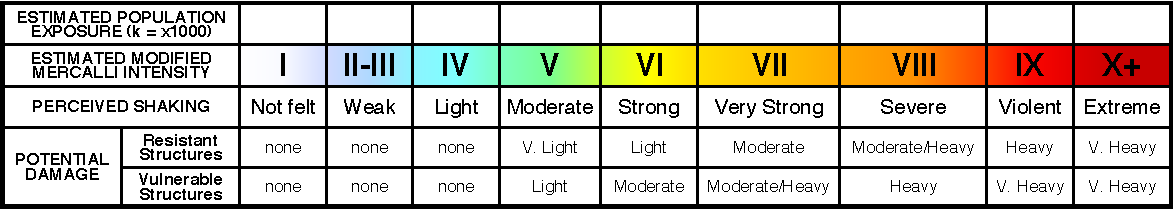
\includegraphics[width=20.05cm]{[HOMEDIR]/losspager/logos/exptable.pdf}
\end{textblock}

\begin{textblock}{1.5}(4.6,8.35)
  \centering [MMI1]
\end{textblock}

\begin{textblock}{1.5}(6.1,8.35)
  \centering [MMI2-3]
\end{textblock}

\begin{textblock}{1.5}(7.6,8.35)
  \centering [MMI4]
\end{textblock}

\begin{textblock}{1.7}(9.1,8.35)
  \centering [MMI5]
\end{textblock}

\begin{textblock}{1.65}(10.8,8.35)
  \centering [MMI6]
\end{textblock}

\begin{textblock}{2.45}(12.45,8.35)
  \centering [MMI7]
\end{textblock}

\begin{textblock}{2.5}(14.9,8.35)
  \centering [MMI8]
\end{textblock}

\begin{textblock}{1.5}(17.4,8.35)
  \centering [MMI9]
\end{textblock}

\begin{textblock}{1.65}(18.9,8.35)
  \centering [MMI10]
\end{textblock}

\begin{textblock}{7.5}(13.4,15.6)
\textbf{Historical Earthquakes (with MMI levels):}
\end{textblock}

\begin{textblock}{6.6}(13.4,16.0)
[HISTORICAL_BLOCK]
\end{textblock}

\begin{textblock}{7.5}(13.4,20.2)
\fontsize{14}{16.8}\textbf{Selected City Exposure}
\end{textblock}

\begin{textblock}{7.5}(13.4,20.7)
{\footnotesize from GeoNames.org}
\end{textblock}


\begin{textblock}{6.6}(13.4,21.05)
[CITYTABLE]
\end{textblock}

\begin{textblock}{13.0}(0.0,26.35)
{\footnotesize PAGER content is automatically generated, and only considers losses due
to structural damage.}
\end{textblock}

\begin{textblock}{12.0}(0.0,26.65)
{\footnotesize Limitations of input data, shaking estimates, and loss models 
may add uncertainty.}
\end{textblock}




\begin{textblock}{7.5}(0.0,27.1)
{\footnotesize \textbf{http://earthquake.usgs.gov/pager}}
\end{textblock}

\begin{textblock}{7.5}(13.1,27.1)
\hfill \textbf{[EVENTID]}
\end{textblock}

\end{document}